% Options for packages loaded elsewhere
\PassOptionsToPackage{unicode}{hyperref}
\PassOptionsToPackage{hyphens}{url}
\PassOptionsToPackage{dvipsnames,svgnames,x11names}{xcolor}
%
\documentclass[
  letterpaper,
  DIV=11,
  numbers=noendperiod]{scrartcl}

\usepackage{amsmath,amssymb}
\usepackage{lmodern}
\usepackage{iftex}
\ifPDFTeX
  \usepackage[T1]{fontenc}
  \usepackage[utf8]{inputenc}
  \usepackage{textcomp} % provide euro and other symbols
\else % if luatex or xetex
  \usepackage{unicode-math}
  \defaultfontfeatures{Scale=MatchLowercase}
  \defaultfontfeatures[\rmfamily]{Ligatures=TeX,Scale=1}
\fi
% Use upquote if available, for straight quotes in verbatim environments
\IfFileExists{upquote.sty}{\usepackage{upquote}}{}
\IfFileExists{microtype.sty}{% use microtype if available
  \usepackage[]{microtype}
  \UseMicrotypeSet[protrusion]{basicmath} % disable protrusion for tt fonts
}{}
\makeatletter
\@ifundefined{KOMAClassName}{% if non-KOMA class
  \IfFileExists{parskip.sty}{%
    \usepackage{parskip}
  }{% else
    \setlength{\parindent}{0pt}
    \setlength{\parskip}{6pt plus 2pt minus 1pt}}
}{% if KOMA class
  \KOMAoptions{parskip=half}}
\makeatother
\usepackage{xcolor}
\setlength{\emergencystretch}{3em} % prevent overfull lines
\setcounter{secnumdepth}{-\maxdimen} % remove section numbering
% Make \paragraph and \subparagraph free-standing
\ifx\paragraph\undefined\else
  \let\oldparagraph\paragraph
  \renewcommand{\paragraph}[1]{\oldparagraph{#1}\mbox{}}
\fi
\ifx\subparagraph\undefined\else
  \let\oldsubparagraph\subparagraph
  \renewcommand{\subparagraph}[1]{\oldsubparagraph{#1}\mbox{}}
\fi

\usepackage{color}
\usepackage{fancyvrb}
\newcommand{\VerbBar}{|}
\newcommand{\VERB}{\Verb[commandchars=\\\{\}]}
\DefineVerbatimEnvironment{Highlighting}{Verbatim}{commandchars=\\\{\}}
% Add ',fontsize=\small' for more characters per line
\usepackage{framed}
\definecolor{shadecolor}{RGB}{241,243,245}
\newenvironment{Shaded}{\begin{snugshade}}{\end{snugshade}}
\newcommand{\AlertTok}[1]{\textcolor[rgb]{0.68,0.00,0.00}{#1}}
\newcommand{\AnnotationTok}[1]{\textcolor[rgb]{0.37,0.37,0.37}{#1}}
\newcommand{\AttributeTok}[1]{\textcolor[rgb]{0.40,0.45,0.13}{#1}}
\newcommand{\BaseNTok}[1]{\textcolor[rgb]{0.68,0.00,0.00}{#1}}
\newcommand{\BuiltInTok}[1]{\textcolor[rgb]{0.00,0.23,0.31}{#1}}
\newcommand{\CharTok}[1]{\textcolor[rgb]{0.13,0.47,0.30}{#1}}
\newcommand{\CommentTok}[1]{\textcolor[rgb]{0.37,0.37,0.37}{#1}}
\newcommand{\CommentVarTok}[1]{\textcolor[rgb]{0.37,0.37,0.37}{\textit{#1}}}
\newcommand{\ConstantTok}[1]{\textcolor[rgb]{0.56,0.35,0.01}{#1}}
\newcommand{\ControlFlowTok}[1]{\textcolor[rgb]{0.00,0.23,0.31}{#1}}
\newcommand{\DataTypeTok}[1]{\textcolor[rgb]{0.68,0.00,0.00}{#1}}
\newcommand{\DecValTok}[1]{\textcolor[rgb]{0.68,0.00,0.00}{#1}}
\newcommand{\DocumentationTok}[1]{\textcolor[rgb]{0.37,0.37,0.37}{\textit{#1}}}
\newcommand{\ErrorTok}[1]{\textcolor[rgb]{0.68,0.00,0.00}{#1}}
\newcommand{\ExtensionTok}[1]{\textcolor[rgb]{0.00,0.23,0.31}{#1}}
\newcommand{\FloatTok}[1]{\textcolor[rgb]{0.68,0.00,0.00}{#1}}
\newcommand{\FunctionTok}[1]{\textcolor[rgb]{0.28,0.35,0.67}{#1}}
\newcommand{\ImportTok}[1]{\textcolor[rgb]{0.00,0.46,0.62}{#1}}
\newcommand{\InformationTok}[1]{\textcolor[rgb]{0.37,0.37,0.37}{#1}}
\newcommand{\KeywordTok}[1]{\textcolor[rgb]{0.00,0.23,0.31}{#1}}
\newcommand{\NormalTok}[1]{\textcolor[rgb]{0.00,0.23,0.31}{#1}}
\newcommand{\OperatorTok}[1]{\textcolor[rgb]{0.37,0.37,0.37}{#1}}
\newcommand{\OtherTok}[1]{\textcolor[rgb]{0.00,0.23,0.31}{#1}}
\newcommand{\PreprocessorTok}[1]{\textcolor[rgb]{0.68,0.00,0.00}{#1}}
\newcommand{\RegionMarkerTok}[1]{\textcolor[rgb]{0.00,0.23,0.31}{#1}}
\newcommand{\SpecialCharTok}[1]{\textcolor[rgb]{0.37,0.37,0.37}{#1}}
\newcommand{\SpecialStringTok}[1]{\textcolor[rgb]{0.13,0.47,0.30}{#1}}
\newcommand{\StringTok}[1]{\textcolor[rgb]{0.13,0.47,0.30}{#1}}
\newcommand{\VariableTok}[1]{\textcolor[rgb]{0.07,0.07,0.07}{#1}}
\newcommand{\VerbatimStringTok}[1]{\textcolor[rgb]{0.13,0.47,0.30}{#1}}
\newcommand{\WarningTok}[1]{\textcolor[rgb]{0.37,0.37,0.37}{\textit{#1}}}

\providecommand{\tightlist}{%
  \setlength{\itemsep}{0pt}\setlength{\parskip}{0pt}}\usepackage{longtable,booktabs,array}
\usepackage{calc} % for calculating minipage widths
% Correct order of tables after \paragraph or \subparagraph
\usepackage{etoolbox}
\makeatletter
\patchcmd\longtable{\par}{\if@noskipsec\mbox{}\fi\par}{}{}
\makeatother
% Allow footnotes in longtable head/foot
\IfFileExists{footnotehyper.sty}{\usepackage{footnotehyper}}{\usepackage{footnote}}
\makesavenoteenv{longtable}
\usepackage{graphicx}
\makeatletter
\def\maxwidth{\ifdim\Gin@nat@width>\linewidth\linewidth\else\Gin@nat@width\fi}
\def\maxheight{\ifdim\Gin@nat@height>\textheight\textheight\else\Gin@nat@height\fi}
\makeatother
% Scale images if necessary, so that they will not overflow the page
% margins by default, and it is still possible to overwrite the defaults
% using explicit options in \includegraphics[width, height, ...]{}
\setkeys{Gin}{width=\maxwidth,height=\maxheight,keepaspectratio}
% Set default figure placement to htbp
\makeatletter
\def\fps@figure{htbp}
\makeatother

\KOMAoption{captions}{tableheading}
\makeatletter
\makeatother
\makeatletter
\makeatother
\makeatletter
\@ifpackageloaded{caption}{}{\usepackage{caption}}
\AtBeginDocument{%
\ifdefined\contentsname
  \renewcommand*\contentsname{Table of contents}
\else
  \newcommand\contentsname{Table of contents}
\fi
\ifdefined\listfigurename
  \renewcommand*\listfigurename{List of Figures}
\else
  \newcommand\listfigurename{List of Figures}
\fi
\ifdefined\listtablename
  \renewcommand*\listtablename{List of Tables}
\else
  \newcommand\listtablename{List of Tables}
\fi
\ifdefined\figurename
  \renewcommand*\figurename{Figure}
\else
  \newcommand\figurename{Figure}
\fi
\ifdefined\tablename
  \renewcommand*\tablename{Table}
\else
  \newcommand\tablename{Table}
\fi
}
\@ifpackageloaded{float}{}{\usepackage{float}}
\floatstyle{ruled}
\@ifundefined{c@chapter}{\newfloat{codelisting}{h}{lop}}{\newfloat{codelisting}{h}{lop}[chapter]}
\floatname{codelisting}{Listing}
\newcommand*\listoflistings{\listof{codelisting}{List of Listings}}
\makeatother
\makeatletter
\@ifpackageloaded{caption}{}{\usepackage{caption}}
\@ifpackageloaded{subcaption}{}{\usepackage{subcaption}}
\makeatother
\makeatletter
\@ifpackageloaded{tcolorbox}{}{\usepackage[many]{tcolorbox}}
\makeatother
\makeatletter
\@ifundefined{shadecolor}{\definecolor{shadecolor}{rgb}{.97, .97, .97}}
\makeatother
\makeatletter
\makeatother
\ifLuaTeX
  \usepackage{selnolig}  % disable illegal ligatures
\fi
\IfFileExists{bookmark.sty}{\usepackage{bookmark}}{\usepackage{hyperref}}
\IfFileExists{xurl.sty}{\usepackage{xurl}}{} % add URL line breaks if available
\urlstyle{same} % disable monospaced font for URLs
\hypersetup{
  pdftitle={Lab 1 - Data visualization},
  pdfauthor={{[}Kaley Sperling{]}},
  colorlinks=true,
  linkcolor={blue},
  filecolor={Maroon},
  citecolor={Blue},
  urlcolor={Blue},
  pdfcreator={LaTeX via pandoc}}

\title{Lab 1 - Data visualization}
\author{{[}Kaley Sperling{]}}
\date{}

\begin{document}
\maketitle
\ifdefined\Shaded\renewenvironment{Shaded}{\begin{tcolorbox}[interior hidden, breakable, boxrule=0pt, sharp corners, enhanced, frame hidden, borderline west={3pt}{0pt}{shadecolor}]}{\end{tcolorbox}}\fi

\hypertarget{load-packages}{%
\subsection{Load Packages}\label{load-packages}}

\begin{Shaded}
\begin{Highlighting}[]
\FunctionTok{library}\NormalTok{(tidyverse)}
\end{Highlighting}
\end{Shaded}

\begin{verbatim}
Warning in system("timedatectl", intern = TRUE): running command 'timedatectl'
had status 1
\end{verbatim}

\begin{Shaded}
\begin{Highlighting}[]
\FunctionTok{library}\NormalTok{(viridis)}
\end{Highlighting}
\end{Shaded}

\hypertarget{exercise-1}{%
\subsection{Exercise 1}\label{exercise-1}}

\begin{Shaded}
\begin{Highlighting}[]
\FunctionTok{glimpse}\NormalTok{(midwest)}
\end{Highlighting}
\end{Shaded}

\begin{verbatim}
Rows: 437
Columns: 28
$ PID                  <int> 561, 562, 563, 564, 565, 566, 567, 568, 569, 570,~
$ county               <chr> "ADAMS", "ALEXANDER", "BOND", "BOONE", "BROWN", "~
$ state                <chr> "IL", "IL", "IL", "IL", "IL", "IL", "IL", "IL", "~
$ area                 <dbl> 0.052, 0.014, 0.022, 0.017, 0.018, 0.050, 0.017, ~
$ poptotal             <int> 66090, 10626, 14991, 30806, 5836, 35688, 5322, 16~
$ popdensity           <dbl> 1270.9615, 759.0000, 681.4091, 1812.1176, 324.222~
$ popwhite             <int> 63917, 7054, 14477, 29344, 5264, 35157, 5298, 165~
$ popblack             <int> 1702, 3496, 429, 127, 547, 50, 1, 111, 16, 16559,~
$ popamerindian        <int> 98, 19, 35, 46, 14, 65, 8, 30, 8, 331, 51, 26, 17~
$ popasian             <int> 249, 48, 16, 150, 5, 195, 15, 61, 23, 8033, 89, 3~
$ popother             <int> 124, 9, 34, 1139, 6, 221, 0, 84, 6, 1596, 20, 7, ~
$ percwhite            <dbl> 96.71206, 66.38434, 96.57128, 95.25417, 90.19877,~
$ percblack            <dbl> 2.57527614, 32.90043290, 2.86171703, 0.41225735, ~
$ percamerindan        <dbl> 0.14828264, 0.17880670, 0.23347342, 0.14932156, 0~
$ percasian            <dbl> 0.37675897, 0.45172219, 0.10673071, 0.48691813, 0~
$ percother            <dbl> 0.18762294, 0.08469791, 0.22680275, 3.69733169, 0~
$ popadults            <int> 43298, 6724, 9669, 19272, 3979, 23444, 3583, 1132~
$ perchsd              <dbl> 75.10740, 59.72635, 69.33499, 75.47219, 68.86152,~
$ percollege           <dbl> 19.63139, 11.24331, 17.03382, 17.27895, 14.47600,~
$ percprof             <dbl> 4.355859, 2.870315, 4.488572, 4.197800, 3.367680,~
$ poppovertyknown      <int> 63628, 10529, 14235, 30337, 4815, 35107, 5241, 16~
$ percpovertyknown     <dbl> 96.27478, 99.08714, 94.95697, 98.47757, 82.50514,~
$ percbelowpoverty     <dbl> 13.151443, 32.244278, 12.068844, 7.209019, 13.520~
$ percchildbelowpovert <dbl> 18.011717, 45.826514, 14.036061, 11.179536, 13.02~
$ percadultpoverty     <dbl> 11.009776, 27.385647, 10.852090, 5.536013, 11.143~
$ percelderlypoverty   <dbl> 12.443812, 25.228976, 12.697410, 6.217047, 19.200~
$ inmetro              <int> 0, 0, 0, 1, 0, 0, 0, 0, 0, 1, 0, 0, 0, 1, 0, 1, 0~
$ category             <chr> "AAR", "LHR", "AAR", "ALU", "AAR", "AAR", "LAR", ~
\end{verbatim}

\begin{Shaded}
\begin{Highlighting}[]
\FunctionTok{ggplot}\NormalTok{(midwest, }\FunctionTok{aes}\NormalTok{(}\AttributeTok{x=}\NormalTok{popdensity)) }\SpecialCharTok{+}
  \FunctionTok{geom\_histogram}\NormalTok{(}\AttributeTok{binwidth=}\DecValTok{10000}\NormalTok{) }\SpecialCharTok{+}
  \FunctionTok{labs}\NormalTok{ (}\AttributeTok{x=}\StringTok{"population density"}\NormalTok{,}
        \AttributeTok{y=}\StringTok{"count"}\NormalTok{,}
        \AttributeTok{title=} \StringTok{"population density by county"}\NormalTok{)}
\end{Highlighting}
\end{Shaded}

\begin{figure}[H]

{\centering 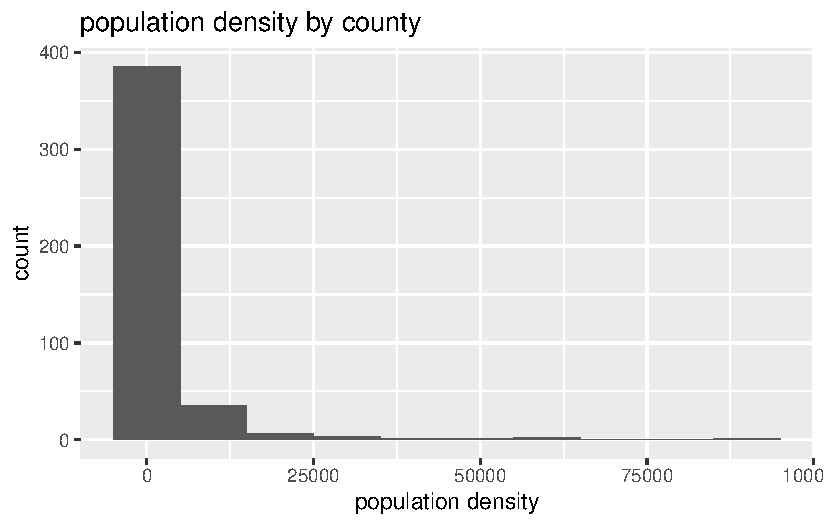
\includegraphics{lab-1_files/figure-pdf/histogram-of-population-density-of-counties-1.pdf}

}

\end{figure}

This is a histogram with a binwidth of 10,000. With this, it is clear to
see the data is right-skewed. There appears to be some sort of outlier
because there are no counties with a population density of 75000 but
there seems to be one with much more than this.

\hypertarget{exercise-2}{%
\subsection{Exercise 2}\label{exercise-2}}

\begin{Shaded}
\begin{Highlighting}[]
\FunctionTok{ggplot}\NormalTok{(midwest, }\FunctionTok{aes}\NormalTok{(}\AttributeTok{x=}\NormalTok{percollege, }\AttributeTok{y=}\NormalTok{percbelowpoverty, }\AttributeTok{color=}\NormalTok{state)) }\SpecialCharTok{+}
  \FunctionTok{geom\_point}\NormalTok{() }\SpecialCharTok{+}
  \FunctionTok{labs}\NormalTok{( }\AttributeTok{x=}\StringTok{"\% college educated"}\NormalTok{,}
    \AttributeTok{y=}\StringTok{"\% below poverty line"}\NormalTok{,}
    \AttributeTok{title=} \StringTok{"\% college educated vs \% below poverty line"}\NormalTok{) }\SpecialCharTok{+}
  \FunctionTok{scale\_color\_viridis\_d}\NormalTok{(}\AttributeTok{option=}\StringTok{"D"}\NormalTok{ )}
\end{Highlighting}
\end{Shaded}

\begin{figure}[H]

{\centering 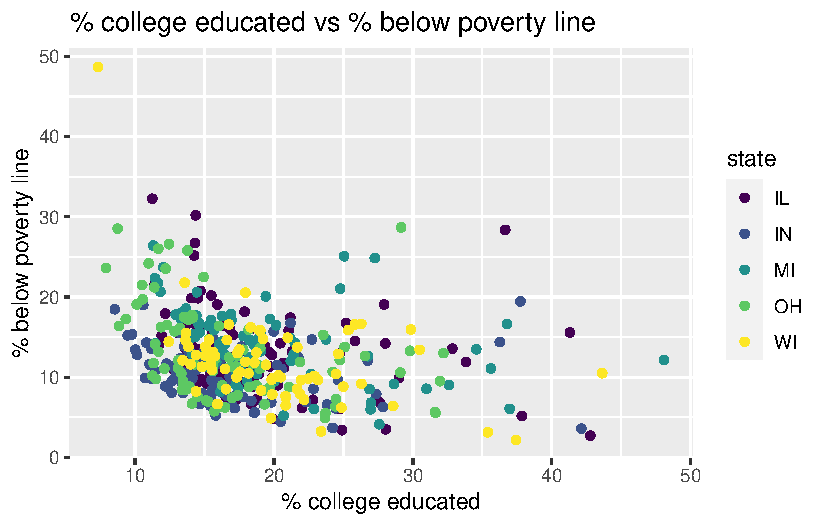
\includegraphics{lab-1_files/figure-pdf/scatterplot-college degree-below-poverty-1.pdf}

}

\end{figure}

\hypertarget{exercise-3}{%
\subsection{Exercise 3}\label{exercise-3}}

In my scatterplot, I can see that the majority of counties in Midwest
states have less than 30\% of their population that are college educated
and less than 20\% below the poverty line. There is one outlier county
in WI where very few people are college educated and nearly 50\% are
below the poverty line. In general, though, Wisconsin has fewer counties
with high percentages of people below the poverty line than other states
in the Midwest.

\hypertarget{exercise-4}{%
\subsection{Exercise 4}\label{exercise-4}}

\begin{Shaded}
\begin{Highlighting}[]
\FunctionTok{ggplot}\NormalTok{(midwest, }\FunctionTok{aes}\NormalTok{(}\AttributeTok{x=}\NormalTok{percollege, }\AttributeTok{y=}\NormalTok{percbelowpoverty, }\AttributeTok{color=}\NormalTok{state)) }\SpecialCharTok{+}
  \FunctionTok{geom\_point}\NormalTok{(}\AttributeTok{alpha=}\FloatTok{0.5}\NormalTok{) }\SpecialCharTok{+}
  \FunctionTok{labs}\NormalTok{( }\AttributeTok{x=}\StringTok{"\% college educated"}\NormalTok{,}
    \AttributeTok{y=}\StringTok{"\% below poverty line"}\NormalTok{,}
    \AttributeTok{title=} \StringTok{"\% college educated vs \% below poverty line"}\NormalTok{) }\SpecialCharTok{+}
  \FunctionTok{scale\_color\_viridis\_d}\NormalTok{(}\AttributeTok{option=}\StringTok{"D"}\NormalTok{ ) }\SpecialCharTok{+}
  \FunctionTok{facet\_wrap}\NormalTok{(}\StringTok{"state"}\NormalTok{) }\SpecialCharTok{+}
  \FunctionTok{geom\_smooth}\NormalTok{(}\AttributeTok{se=}\ConstantTok{FALSE}\NormalTok{, }\AttributeTok{color=}\StringTok{"black"}\NormalTok{)}
\end{Highlighting}
\end{Shaded}

\begin{verbatim}
`geom_smooth()` using method = 'loess' and formula 'y ~ x'
\end{verbatim}

\begin{figure}[H]

{\centering 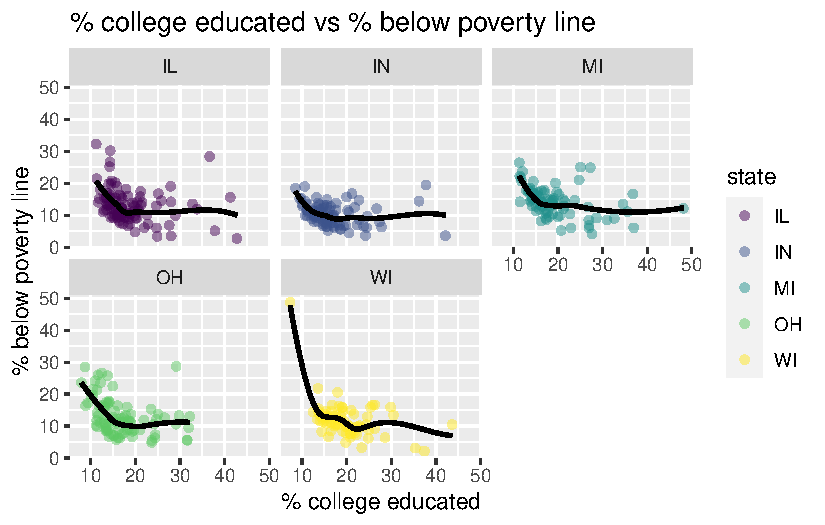
\includegraphics{lab-1_files/figure-pdf/separate-scatter-for-each-state-1.pdf}

}

\end{figure}

I much prefer this plot. It makes it easier to see the overall pattern
and therefore relationship between the two variables. Also, the data by
state is no longer on top of one another.

\hypertarget{exercise-5}{%
\subsection{Exercise 5}\label{exercise-5}}

\begin{Shaded}
\begin{Highlighting}[]
\FunctionTok{ggplot}\NormalTok{(midwest, }\FunctionTok{aes}\NormalTok{(}\AttributeTok{x=}\NormalTok{area)) }\SpecialCharTok{+} 
  \FunctionTok{geom\_boxplot}\NormalTok{() }\SpecialCharTok{+}
  \FunctionTok{facet\_wrap}\NormalTok{(}\StringTok{"state"}\NormalTok{)}
\end{Highlighting}
\end{Shaded}

\begin{figure}[H]

{\centering \includegraphics{lab-1_files/figure-pdf/areas-of-counties-by-state\}-1.pdf}

}

\end{figure}

It seems that some states have larger county areas than others. On
average (Q2), counties in WI have the more area than other states.
However, Michigan has the county with the largest area in the Midwest. I
can tell because the tail in Q4, the last data point, is the furthest to
the right for MI.

\hypertarget{exercise-6}{%
\subsection{Exercise 6}\label{exercise-6}}

\begin{Shaded}
\begin{Highlighting}[]
\NormalTok{ midwest }\OtherTok{\textless{}{-}}\NormalTok{ midwest }\SpecialCharTok{|\textgreater{}} 
   \FunctionTok{mutate}\NormalTok{(}\AttributeTok{metro =} \FunctionTok{if\_else}\NormalTok{(inmetro }\SpecialCharTok{==} \DecValTok{1}\NormalTok{, }\StringTok{"Yes"}\NormalTok{, }\StringTok{"No"}\NormalTok{))}
 \FunctionTok{ggplot}\NormalTok{(midwest, }\FunctionTok{aes}\NormalTok{(}\AttributeTok{x=}\NormalTok{state,}\AttributeTok{fill=}\NormalTok{metro)) }\SpecialCharTok{+}
   \FunctionTok{geom\_bar}\NormalTok{(}\AttributeTok{position=}\StringTok{"fill"}\NormalTok{) }\SpecialCharTok{+}
   \FunctionTok{labs}\NormalTok{( }\AttributeTok{x=}\StringTok{"state"}\NormalTok{,}
    \AttributeTok{y=}\StringTok{"\% metro"}\NormalTok{,}
    \AttributeTok{title=} \StringTok{"\% of counties in metro areas"}\NormalTok{)}
\end{Highlighting}
\end{Shaded}

\begin{figure}[H]

{\centering \includegraphics{lab-1_files/figure-pdf/percentage-of-counties-in-metro-areas\}-1.pdf}

}

\end{figure}

I notice that Ohio and Indiana have the most counties in metropolitan
areas and Wisconsin and Illinois have the least.

\hypertarget{exercise-7}{%
\subsection{Exercise 7}\label{exercise-7}}



\end{document}
